\section{Evaluation}

\subsection{Overview}

This section evaluates the performance, reliability, and transparency of the proposed signal generation and recommendation framework. We begin with a quantitative analysis of the model’s classification accuracy, consistency across market conditions, and outcome alignment. This is followed by an interpretability study leveraging SHAP values to understand the influence of individual input features. We also examine the quality and usefulness of natural language explanations generated by a local LLM, supported by a manual annotation template. The evaluation concludes with a discussion of current limitations and an overall assessment of the system’s strengths and areas for further refinement.

\subsection{Evaluation Design}
The evaluation process was grounded in the incremental development of the system. As the MVP expanded from a single-indicator engine (SMA crossover) to a modular, ensemble-based architecture, the system was structured to support isolated testing of each signal module. Indicators such as RSI and MACD were added as independent Python modules, allowing for precise attribution and targeted validation.

This modular design also enabled a batch evaluation process, in which the system was tested across multiple tickers and historical timestamps using a strict cut-off methodology. Outputs—including recommendations, explanations, and realised price changes—were logged to structured CSV files. These formed the basis for subsequent analysis.

Supporting Jupyter notebooks were developed to visualise the relationship between recommendation types and price movement outcomes. Visual tools such as histograms and boxplots were used to inspect signal performance, and early empirical trends (e.g., the hit rate of BUY signals) informed further refinement of strategy logic and prompt design.

\subsection{Methodology}

The evaluation employed a cut-off-based backtesting framework to simulate the system’s recommendations in a temporally realistic setting. For each ticker, historical data was truncated at a fixed cut-off date, beyond which no future information was accessible to the strategy engine. A 30-day lookahead horizon was then used to observe forward price movements and assess the quality of the generated recommendation.

Batch evaluations were conducted across a curated list of generative AI-related equities and multiple monthly cut-off dates. This enabled temporal robustness checks and cross-sectional analysis of the model’s behaviour. To ensure determinism and reproducibility, all equity data was fetched from local CSV caches generated during prior ingestion runs, thereby avoiding API variability or data drift.

This methodology allowed for an ex-post evaluation of the advisory system while respecting realistic information boundaries and supporting statistical aggregation across time and instruments.

\subsection{Implementation of the Backtesting Pipeline}

The backtesting pipeline was implemented as a modular Python batch system. Its core function, \texttt{backtest\_ticker()}, accepts a stock ticker and a historical cut-off date as input. It slices the cached price data to include only records available up to that date, thereby simulating a realistic information boundary. A composite recommendation is generated using the ensemble strategy engine, and an accompanying explanation is produced via the local language model.

To assess recommendation performance, the system fetches post-cutoff price data over a fixed lookahead horizon (30 days), and calculates the forward percentage return. The results are compiled into structured dictionaries containing the ticker, as-of date, recommendation, rationale, explanation, and forward price change. This design ensures strict temporal separation between signal generation and performance evaluation, eliminating data leakage.

A higher-level orchestration script, \texttt{batch\_backtesting.py}, automates this process over multiple tickers and dates. It reads tickers from a CSV watchlist and iterates through a configurable set of evaluation dates. Outputs from each backtest run are logged to timestamped CSV files in a dedicated evaluation directory, enabling reproducibility and version tracking.

The resulting datasets are subsequently explored using Jupyter notebooks. These notebooks facilitate performance visualisation, signal attribution, and exploratory metrics computation. This architecture supports both batch scalability and transparent post hoc analysis.

\subsection{Quantitative Signal Performance}

This subsection evaluates the predictive efficacy of the system's generated trading signals—BUY, HOLD, and SELL—using both statistical visualisation and classification metrics.

\paragraph{Distribution Analysis.}  
The violin and box plots (Figures~\ref{fig:violin} and~\ref{fig:box}) show the distribution of 30-day forward price changes conditioned on the system’s recommendations. The SELL group exhibits the most left-skewed distribution, indicating that negative returns were most prevalent following these signals. 

\begin{figure}[h]
  \centering
  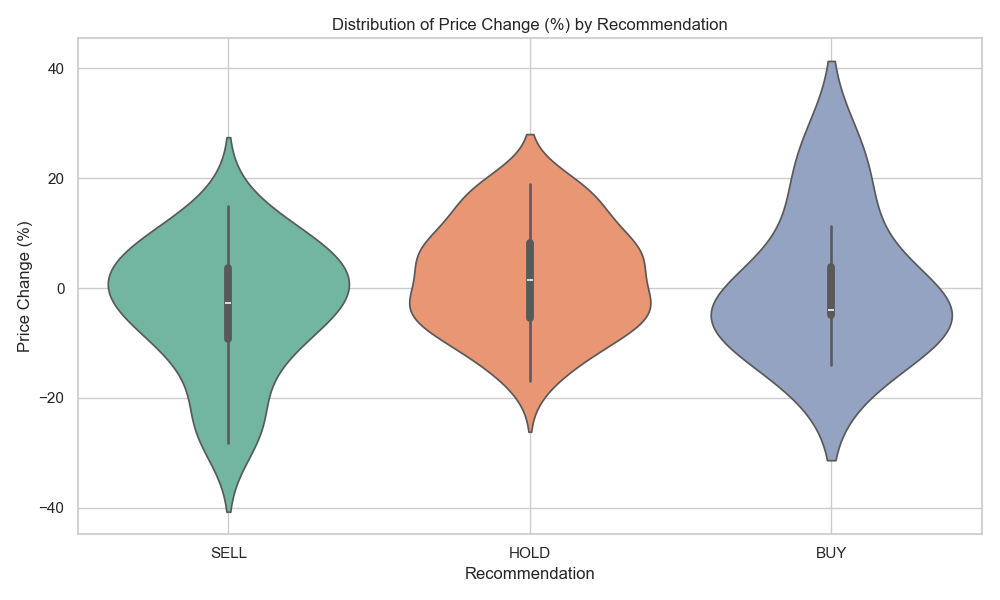
\includegraphics[width=0.6\linewidth]{assets/violin_plot.png}
  \caption{Distribution of Price Change (\%) by Recommendation Type}
  \label{fig:violin}
\end{figure}

\begin{figure}[h]
  \centering
  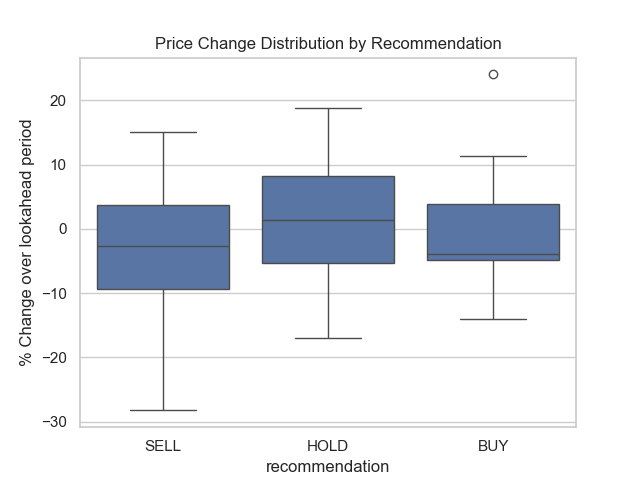
\includegraphics[width=0.6\linewidth]{assets/price_change_distribution_by_recommendation.png}
  \caption{Boxplot of Price Change by Recommendation}
  \label{fig:box}
\end{figure}

\FloatBarrier

Conversely, the BUY group shows a higher tail on the positive side, albeit with greater dispersion. HOLD recommendations, which dominate the output distribution (see Figure~\ref{fig:rec_dist}), tend to centre around zero return, aligning with the system's intent to recommend HOLD in uncertain or balanced cases.

\begin{figure}[h]
  \centering
  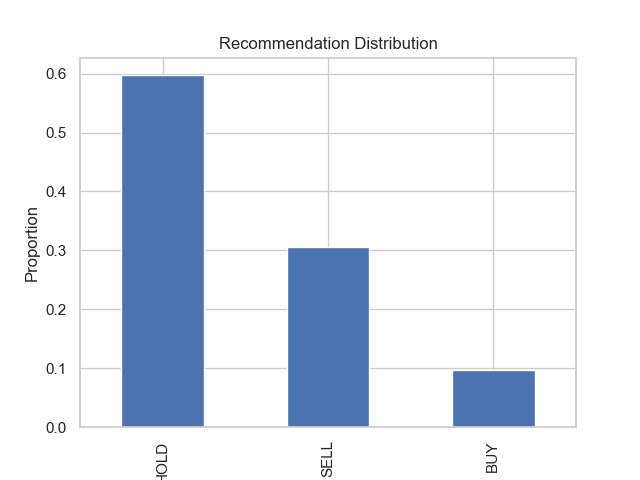
\includegraphics[width=0.6\linewidth]{assets/recommendation_distribution.png}
  \caption{Recommendation Type Distribution}
  \label{fig:rec_dist}
\end{figure}

\paragraph{Recommendation Frequency.}  
Figure~\ref{fig:rec_dist} illustrates the proportion of recommendations. HOLD signals dominate, comprising nearly 60\% of total outputs, followed by SELL and then BUY. This asymmetry could stem from conservative aggregation logic in the signal fusion engine or class imbalance during model training.

\paragraph{Prediction Accuracy and Confusion Matrix.}  
Performance metrics derived from backtest outcomes are summarised using a confusion matrix  and classification report (Figure~\ref{fig:confusion-matrix} and Table~\ref{tab:classification-report}). HOLD shows high recall (0.80), indicating the system often correctly predicts when no significant directional movement is expected. However, BUY and SELL classes suffer from lower recall, suggesting many directional changes are incorrectly classified as HOLD. Precision is highest for SELL (0.55), which implies a relatively high proportion of SELL predictions are correct.

\begin{table}[htbp]
\centering
\caption{Classification report by recommendation type}
\label{tab:classification-report}
\begin{tabular}{lccc}
\hline
\textbf{Class} & \textbf{precision} & \textbf{recall} & \textbf{f1-score} \\
\hline
SELL & 0.55 & 0.34 & 0.42 \\
HOLD & 0.09 & 0.80 & 0.17 \\
BUY  & 0.29 & 0.06 & 0.10 \\
\hline
\end{tabular}
\end{table}

\FloatBarrier

\paragraph{Outcome Breakdown.}  
Figure~\ref{fig:outcome_breakdown} details how often each recommendation led to correct, incorrect, or neutral outcomes. Most HOLDs are neutral, while SELLs are more likely to be correct than incorrect. BUY signals remain underrepresented and less accurate, warranting further tuning.

\begin{figure}[h]
  \centering
  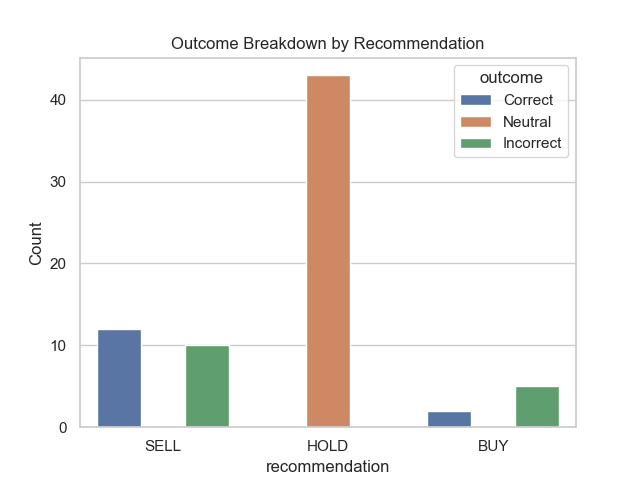
\includegraphics[width=0.6\linewidth]{assets/outcome_breakdown_by_recommendation.png}
  \caption{Outcome Breakdown by Recommendation Type}
  \label{fig:outcome_breakdown}
\end{figure}

Overall, the model demonstrates competent neutral positioning, but directional recommendations require refinement—particularly in improving recall for BUY signals and balancing class representation in both training and orchestration stages.

\subsection{Machine Learning Interpretability}

To provide insight into the decision-making process of the TensorFlow-based classifier, we employed SHAP (SHapley Additive exPlanations) values as a post hoc interpretability technique. SHAP values help attribute the contribution of each feature towards the model’s output in a consistent and theoretically grounded manner.

\begin{figure}[h]
  \centering
  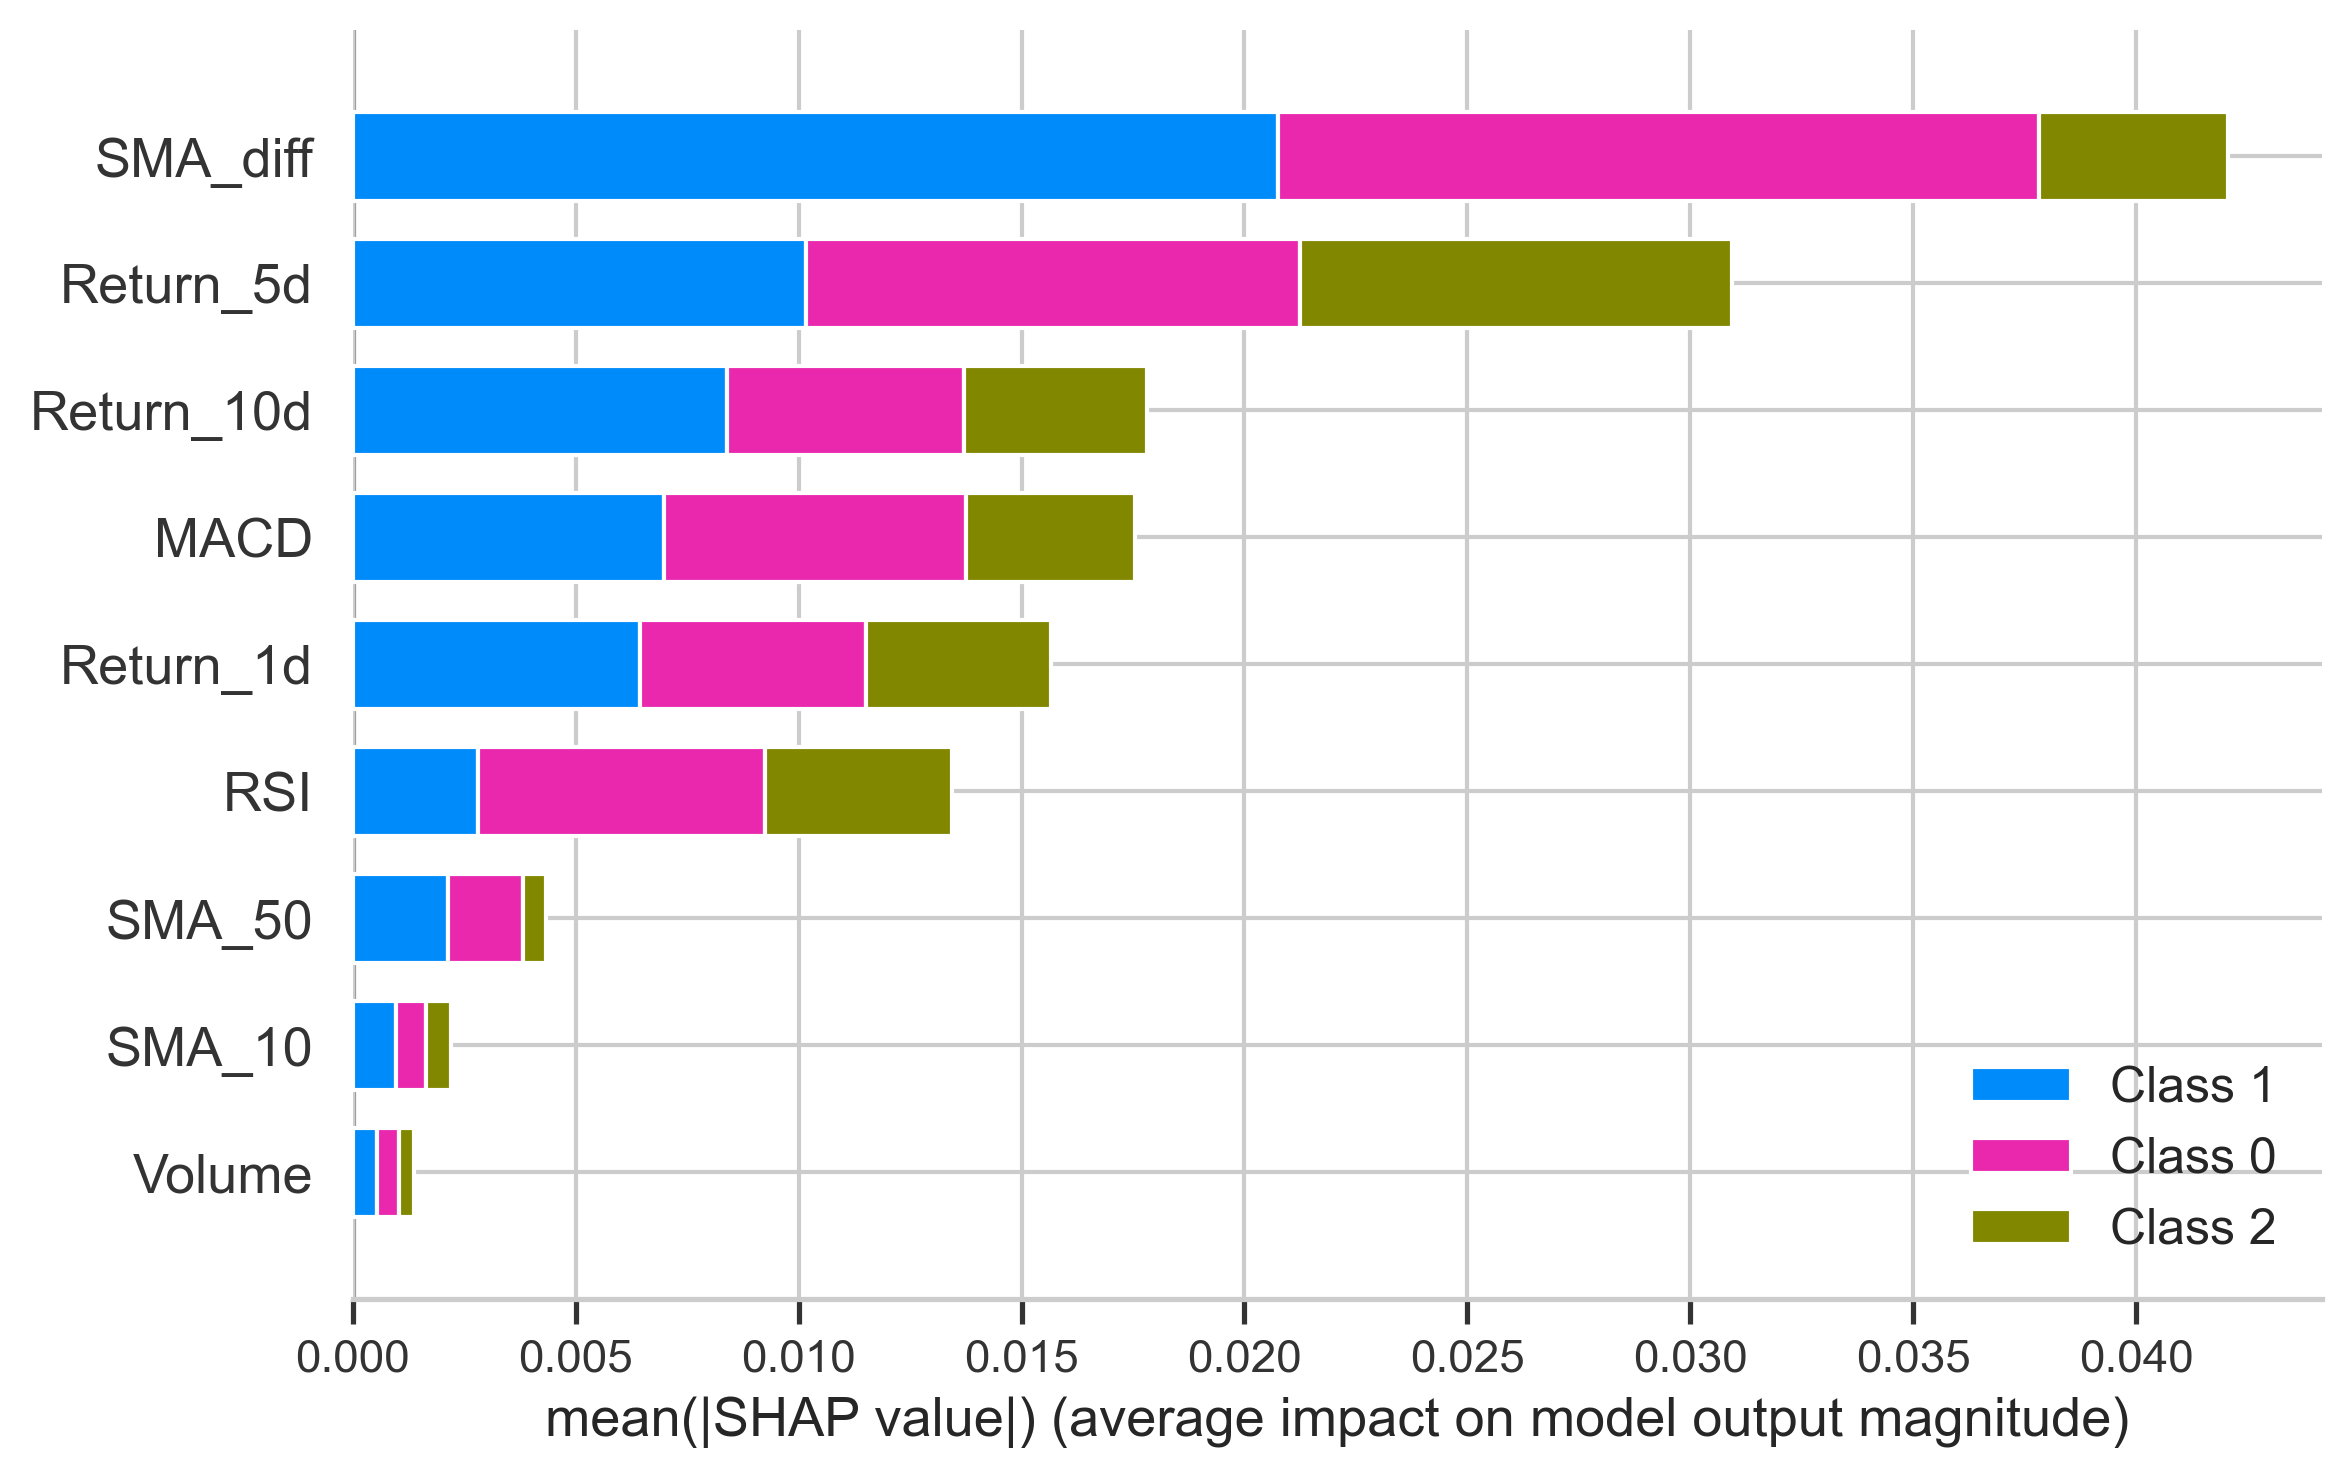
\includegraphics[width=0.8\linewidth]{assets/shap_summary_bar.png}
  \caption{SHAP Summary Plot Showing Average Feature Impact per Class}
  \label{fig:shap_summary}
\end{figure}

Figure~\ref{fig:shap_summary} illustrates the average absolute SHAP values across the three output classes—SELL (0), HOLD (1), and BUY (2). These values indicate the magnitude of impact each input feature has on the model's predictions, averaged across a sample of recent AAPL data points.

The results highlight the dominant role of short- to medium-term technical indicators. In particular, \texttt{SMA\_diff} (the difference between the 10-day and 50-day simple moving averages) exerts the greatest influence across all classes. This suggests the model heavily relies on trend momentum for directional prediction. Return-based features (\texttt{Return\_1d}, \texttt{Return\_5d}, \texttt{Return\_10d}) and \texttt{MACD} also play substantial roles, especially in distinguishing BUY signals. Conversely, features such as \texttt{Volume} and \texttt{SMA\_10} appear to contribute minimally.

Overall, the SHAP analysis reveals that the model bases its forecasts on interpretable technical signals rather than obscure patterns. This reinforces confidence in the model's behaviour, offering transparency critical for user trust in financial decision support systems.

\subsection{Evaluation of Explanations}

To evaluate the effectiveness and clarity of the explanations generated by the large language model (LLM) for each recommendation, we conducted a structured manual assessment. The objective was to determine whether these natural language explanations enhance the transparency and interpretability of the machine learning (ML) predictions, particularly for end-users with financial domain expertise.

Each explanation accompanying a predicted signal (BUY, HOLD, or SELL) was reviewed independently across several qualitative dimensions. These dimensions were selected to reflect the dual requirements of technical correctness and human interpretability. For consistency, all evaluations used the following rubric:

\begin{table}[h]
  \centering
  \caption{Manual Evaluation Template for LLM Explanations}
  \label{tab:llm_eval_template}
  \begin{tabular}{|p{0.18\linewidth}|p{0.12\linewidth}|p{0.58\linewidth}|}
    \hline
    \textbf{Criterion} & \textbf{Score (1–5)} & \textbf{Notes} \\
    \hline
    Relevance &  & Does the explanation directly relate to the input features or context influencing the recommendation? \\
    \hline
    Specificity &  & Is the explanation tailored to the specific case, or does it contain vague or generic language? \\
    \hline
    Correctness &  & Are the financial and technical statements accurate based on the model's behaviour? \\
    \hline
    Interpretability &  & Is the explanation understandable to a non-technical financial analyst or user? \\
    \hline
    Justifiability &  & Does the explanation appear to align with known signals or the model’s inferred logic (e.g., SHAP insights)? \\
    \hline
    Actionability &  & Would the explanation help an analyst or investor make a better-informed decision? \\
    \hline
  \end{tabular}
\end{table}
\FloatBarrier

Table~\ref{tab:llm_eval_template} serves as the structured rubric used to systematically assess the quality of natural language explanations generated by the LLM. Each row corresponds to a key evaluation dimension, and annotators assign a score from 1 (poor) to 5 (excellent), alongside qualitative notes. This ensures that evaluations are not ad hoc, but instead guided by consistent criteria capturing both technical correctness (e.g., accuracy of financial reasoning) and human factors (e.g., clarity and actionability). By enforcing a uniform framework, the template enables transparent comparison across multiple explanations, facilitates reproducibility of results, and highlights recurring strengths and weaknesses in the generated narratives.

\vspace{0.5cm}

\noindent
\textbf{Example Evaluation Entry:}

\begin{itemize}
  \item \textbf{Ticker:} AAPL  
  \item \textbf{Date:} 2025-07-01  
  \item \textbf{Recommendation:} BUY  
  \item \textbf{LLM Explanation:} "The model predicts a BUY signal due to a strong positive MACD crossover, increasing 5-day returns, and rising RSI, all indicating bullish momentum."
  \item \textbf{Evaluator Comments:} The explanation is clear, accurate, and tailored. It could be improved by including model confidence or a mention of recent volatility.
\end{itemize}

\medskip

Evaluations using this framework revealed that while most explanations were interpretable and relevant, some lacked depth in justifiability or failed to clearly connect the language to the underlying numerical signals. In future iterations, incorporating SHAP-derived insights into the explanation prompt may improve quality and consistency across recommendations.

\subsection{Frontend Evaluation}

To ensure accessibility and user engagement, the GenAI Advisor features an interactive web-based frontend built with Streamlit. The application is structured around two primary views: the portfolio-level overview and the detailed ticker analysis, each designed to support both technical users and novices seeking intuitive insights.

\paragraph{Portfolio Overview}
Figure~\ref{fig:ui_portfolio} shows the application’s landing view, where all GenAI-related companies are automatically analysed. Each row displays a ticker symbol, its full name, the current recommendation (BUY, HOLD, or SELL), and a succinct reason summarising the signal consensus. This view is designed for a fast scan of the market sentiment across the watchlist.

\begin{figure}[h]
\centering
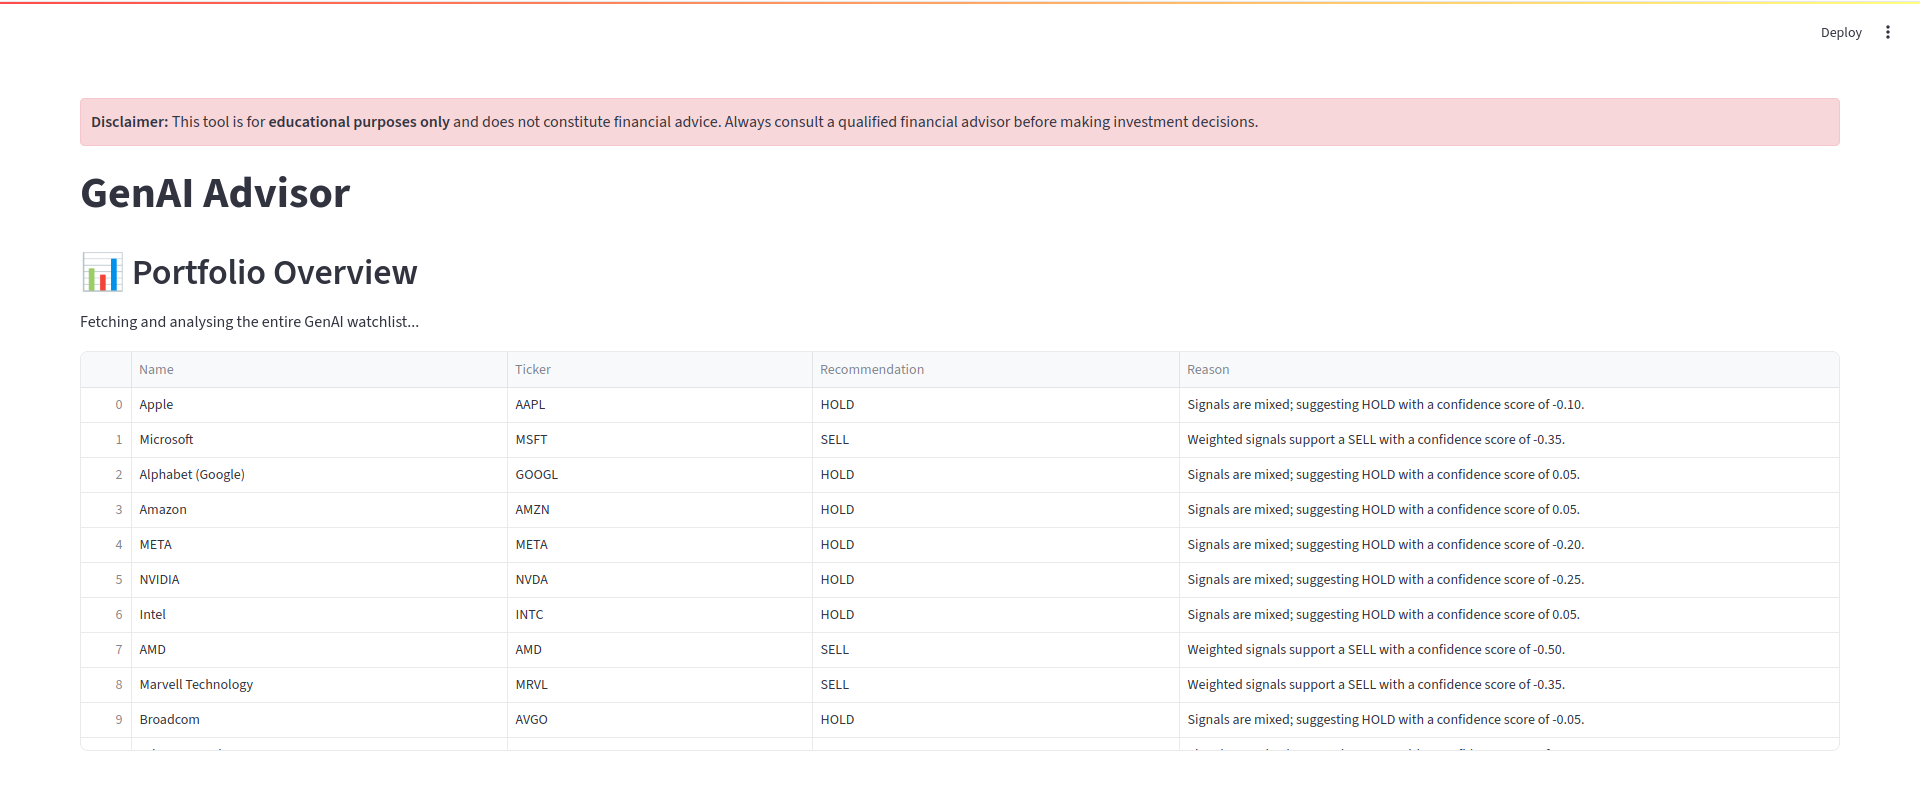
\includegraphics[width=0.9\linewidth]{assets/ui1-portfolio_overview.png}
\caption{Portfolio-Level Recommendation Summary}
\label{fig:ui_portfolio}
\end{figure}

\paragraph{Detailed Ticker Analysis}
Upon selecting a specific company, users are presented with a more granular analysis panel (Figure~\ref{fig:ui_detailed}). The system fetches historical stock data (defaulting to 10 years) and visualises the price trend. Subsequently, a hybrid strategy engine computes the combined recommendation, which is further broken down into individual signal components. Each indicator—such as SMA crossover, RSI, MACD, Bollinger Bands, and others—contributes an individual recommendation with a natural language justification.

\begin{figure}[h]
\centering
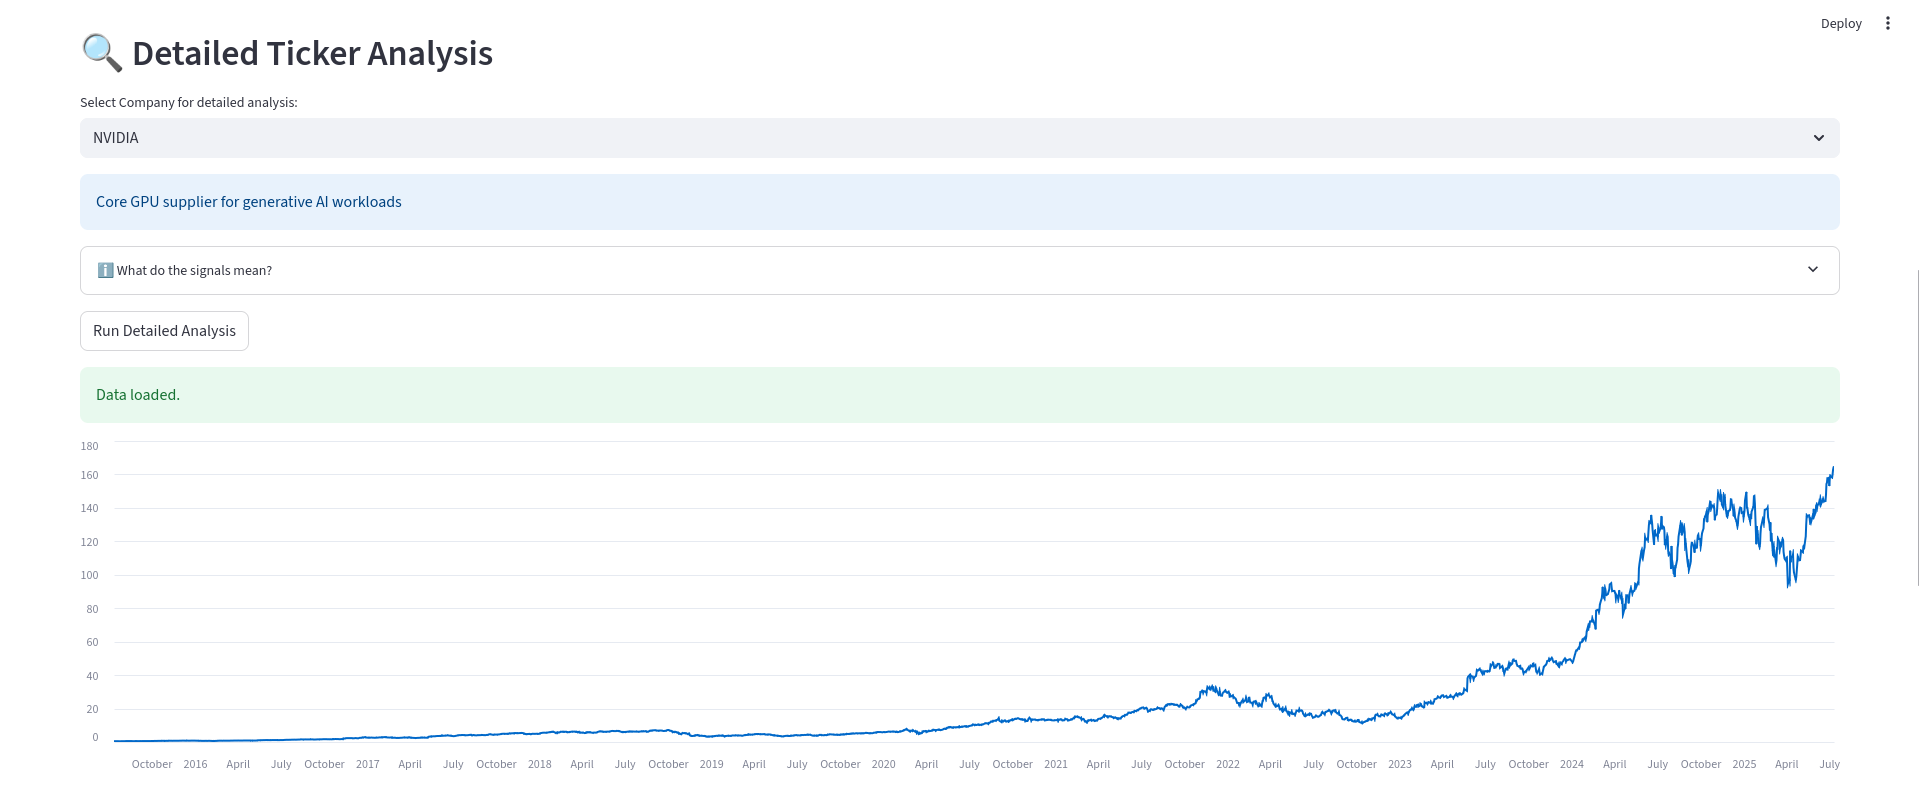
\includegraphics[width=0.9\linewidth]{assets/ui2-ticker_analysis.png}
\caption{Detailed Ticker Analysis View}
\label{fig:ui_detailed}
\end{figure}

\paragraph{Explanation Generation and Export}
Figure~\ref{fig:ui_explanation} showcases the final segment of the analysis: a large language model (LLM)-generated explanation that contextualises the decision. The system measures and displays the explanation latency, stores the interaction in a log file, and allows users to download a PDF report for offline review or sharing. The inclusion of export functionality and speed metrics enhances both usability and transparency.

\begin{figure}[h]
\centering
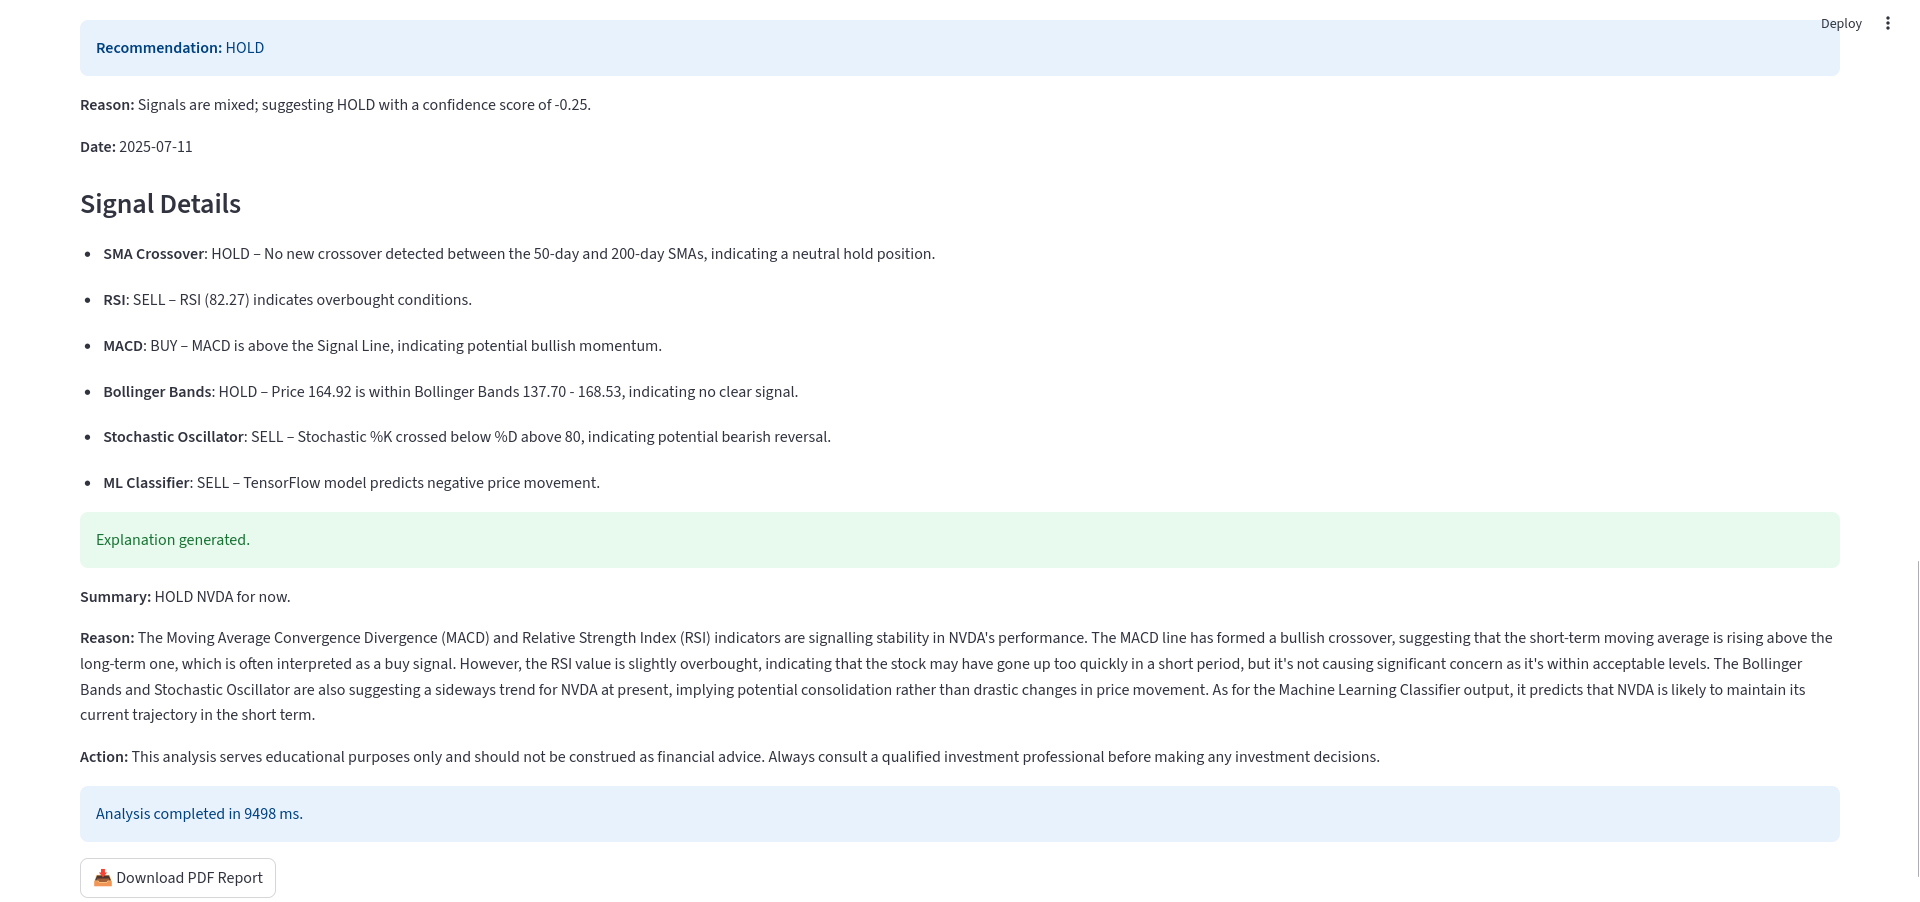
\includegraphics[width=0.9\linewidth]{assets/ui3-explanation.png}
\caption{Model Explanation, Signal Breakdown, and Export Features}
\label{fig:ui_explanation}
\end{figure}

\FloatBarrier

\paragraph{User Experience Considerations}
The frontend emphasises clarity and educational value. Tooltips, expandable signal descriptions, and consistent colour schemes help guide the user. Furthermore, a disclaimer is persistently shown to remind users that the tool is intended strictly for educational use and does not replace professional financial advice.

Overall, the frontend complements the backend analytics by delivering insights in an accessible, trustworthy, and aesthetically clean format.

\paragraph{Limitations.}  
Some latency spikes may occur when the local LLM (e.g., Mistral) is under GPU memory contention, or if data retrieval is delayed. Additionally, the current application design assumes end-users are familiar with basic financial concepts, which may limit accessibility for novices.

\paragraph{Future Enhancements}  
Planned improvements include persistent user session logging, mobile responsiveness, SHAP visualisation integration, and model versioning metadata in downloadable reports.

\subsection{Limitations}

Despite the promising performance and comprehensive evaluation of the machine learning (ML) signal generation and explanation pipeline, several limitations must be acknowledged.

\paragraph{Model Performance and Generalisation.}  
The TensorFlow-based classifier demonstrates moderate performance, especially in correctly identifying BUY signals, which remain underrepresented and less accurate compared to SELL and HOLD. This class imbalance introduces bias into the model and limits its generalisability to unseen or volatile market conditions. While class weights and data augmentation were partially addressed, further refinement is required to balance predictive power across all classes.

\paragraph{Data Scope and Market Conditions.}  
The training data is based on historical daily prices of a limited set of US technology stocks over a 10-year period. This constraint may reduce the model’s robustness to macroeconomic shifts, structural breaks, or non-tech sector behaviours. The use of fixed lookback and forecast horizons may also fail to capture dynamics with varying time lags or temporal dependencies.

\paragraph{Explanation Fidelity.}  
Although SHAP values provide local interpretability and the LLM-generated narratives offer human-readable justifications, the explanations may not always faithfully represent the underlying model mechanics. SHAP explanations are based on approximations and are sensitive to input distributions and feature correlation. Meanwhile, the LLM explanations—while fluent—may introduce hallucinations or overstate causal relationships unless tightly grounded in model outputs.

\paragraph{Subjectivity in Manual Evaluation.}  
The assessment of explanation quality relies on human judgement, which introduces subjectivity and potential inconsistencies across reviewers. While the evaluation rubric helps standardise criteria, different levels of domain expertise may influence scoring and interpretation.

\paragraph{Resource Constraints.}  
The interpretability pipeline, especially SHAP computation for deep learning models, remains computationally expensive and was limited to a subset of 100 samples per ticker. This restricts the breadth of explanation analysis and may obscure insights that emerge in longer-term or higher-volume applications.

\paragraph{Absence of Real-Time Testing.}  
All results reported are based on historical backtesting. The model has not yet been deployed in a live market environment where slippage, transaction costs, and execution latency would impact real-world performance. Without live validation, claims of profitability or decision support remain speculative.

\bigskip

Addressing these limitations in future work will be essential for enhancing the system’s reliability, fairness, and operational viability in real-world financial decision-making.

\subsection{Summary}

This section presented a comprehensive evaluation of the machine learning-based recommendation system, combining both quantitative signal performance and interpretability analysis. Through statistical backtesting, confusion matrices, and classification metrics, we assessed the model’s predictive capabilities and identified areas for improvement, particularly in generating BUY signals.

We further examined the system’s interpretability using SHAP values to uncover the most influential input features and evaluated the clarity and quality of the LLM-generated natural language explanations using a structured manual rubric.

While the framework shows promise, several limitations persist, including class imbalance, the scope of training data, and the computational cost of interpretability methods. Despite these, the combination of transparent model insights and explainable recommendations provides a solid foundation for iterative refinement and potential deployment in real-world financial advisory contexts.
